\documentclass[a4paper,14pt,oneside,final]{extarticle}
\usepackage[top=2cm, bottom=2cm, left=3cm, right=1cm]{geometry}
\usepackage{scrextend}

\usepackage[T2A,T1]{fontenc}
\usepackage[ukrainian,russian,english]{babel}
\usepackage{tempora}
\usepackage{fontspec}
\setmainfont{tempora}

% Зачем: Отключает использование изменяемых межсловных пробелов.
% Почему: Так не принято делать в текстах на русском языке.
\frenchspacing

\usepackage{indentfirst}
\setlength{\parindent}{1.25cm}
\renewcommand{\baselinestretch}{1.5}

% Header
\usepackage{fancyhdr}
\pagestyle{fancy}
\fancyhead{}
\fancyfoot{}
\fancyhead[R]{\small \selectfont \thepage}
\renewcommand{\headrulewidth}{0pt}

% Captions
\usepackage{chngcntr}
\counterwithin{figure}{section}
\counterwithin{table}{section}
\usepackage[tableposition=top]{caption}
\usepackage{subcaption}
\DeclareCaptionLabelFormat{gostfigure}{Рисунок #2}
\DeclareCaptionLabelFormat{gosttable}{Таблиця #2}
\DeclareCaptionLabelSeparator{gost}{~---~}
\captionsetup{labelsep=gost}
\captionsetup[figure]{labelformat=gostfigure}
\captionsetup[table]{labelformat=gosttable}
\renewcommand{\thesubfigure}{\asbuk{subfigure}}

% Sections
\usepackage[explicit]{titlesec}
\newcommand{\sectionbreak}{\clearpage}

\titleformat{\section}
  {\centering}{\thesection \quad}{0pt}{\MakeUppercase{#1}}
\titleformat{\subsection}[block]
  {\bfseries}{\thesubsection \quad #1}{0cm}{}

\titlespacing{\section} {0cm}{0cm}{21pt}
\titlespacing{\subsection} {\parindent}{21pt}{0cm}
\titlespacing{\subsubsection} {\parindent}{0cm}{0cm}

% Lists
\usepackage{enumitem}
\renewcommand\labelitemi{--}
\setlist[itemize]{noitemsep, topsep=0pt, wide}
\setlist[enumerate]{noitemsep, topsep=0pt, wide, label=\arabic*}
\setlist[description]{labelsep=0pt, noitemsep, topsep=0pt, leftmargin=2\parindent, labelindent=\parindent, labelwidth=\parindent, font=\normalfont}

% Toc
\usepackage{tocloft}
\tocloftpagestyle{fancy}
\renewcommand{\cfttoctitlefont}{}
\setlength{\cftbeforesecskip}{0pt}
\renewcommand{\cftsecfont}{}
\renewcommand{\cftsecpagefont}{}
\renewcommand{\cftsecleader}{\cftdotfill{\cftdotsep}}

\usepackage{float}
\usepackage{pgfplots}
\usepackage{graphicx}
\usepackage{multirow}
\usepackage{amssymb,amsfonts,amsmath,amsthm}
\usepackage{csquotes}

\usepackage{listings}
\lstset{basicstyle=\footnotesize\ttfamily,breaklines=true}
\lstset{language=Matlab}

\usepackage[
	backend=biber,
	sorting=none,
	language=auto,
	autolang=other
]{biblatex}
\DeclareFieldFormat{labelnumberwidth}{#1}


\newcommand{\labnumber}{4} % fourth lab
\documentclass[a4paper,14pt,oneside,final]{extarticle}
\usepackage[top=2cm, bottom=2cm, left=3cm, right=1cm]{geometry}
\usepackage{scrextend}

\usepackage[T2A,T1]{fontenc}
\usepackage[ukrainian,russian,english]{babel}
\usepackage{tempora}
\usepackage{fontspec}
\setmainfont{tempora}

% Зачем: Отключает использование изменяемых межсловных пробелов.
% Почему: Так не принято делать в текстах на русском языке.
\frenchspacing

\usepackage{indentfirst}
\setlength{\parindent}{1.25cm}
\renewcommand{\baselinestretch}{1.5}

% Header
\usepackage{fancyhdr}
\pagestyle{fancy}
\fancyhead{}
\fancyfoot{}
\fancyhead[R]{\small \selectfont \thepage}
\renewcommand{\headrulewidth}{0pt}

% Captions
\usepackage{chngcntr}
\counterwithin{figure}{section}
\counterwithin{table}{section}
\usepackage[tableposition=top]{caption}
\usepackage{subcaption}
\DeclareCaptionLabelFormat{gostfigure}{Рисунок #2}
\DeclareCaptionLabelFormat{gosttable}{Таблиця #2}
\DeclareCaptionLabelSeparator{gost}{~---~}
\captionsetup{labelsep=gost}
\captionsetup[figure]{labelformat=gostfigure}
\captionsetup[table]{labelformat=gosttable}
\renewcommand{\thesubfigure}{\asbuk{subfigure}}

% Sections
\usepackage[explicit]{titlesec}
\newcommand{\sectionbreak}{\clearpage}

\titleformat{\section}
  {\centering}{\thesection \quad}{0pt}{\MakeUppercase{#1}}
\titleformat{\subsection}[block]
  {\bfseries}{\thesubsection \quad #1}{0cm}{}

\titlespacing{\section} {0cm}{0cm}{21pt}
\titlespacing{\subsection} {\parindent}{21pt}{0cm}
\titlespacing{\subsubsection} {\parindent}{0cm}{0cm}

% Lists
\usepackage{enumitem}
\renewcommand\labelitemi{--}
\setlist[itemize]{noitemsep, topsep=0pt, wide}
\setlist[enumerate]{noitemsep, topsep=0pt, wide, label=\arabic*}
\setlist[description]{labelsep=0pt, noitemsep, topsep=0pt, leftmargin=2\parindent, labelindent=\parindent, labelwidth=\parindent, font=\normalfont}

% Toc
\usepackage{tocloft}
\tocloftpagestyle{fancy}
\renewcommand{\cfttoctitlefont}{}
\setlength{\cftbeforesecskip}{0pt}
\renewcommand{\cftsecfont}{}
\renewcommand{\cftsecpagefont}{}
\renewcommand{\cftsecleader}{\cftdotfill{\cftdotsep}}

\newcommand{\khpistudentgroup}{КН-34г}
\newcommand{\khpistudentname}{Чепурний~А.~С.}

\newcommand{\khpidepartment}{Програмна інженерія та інформаційні технології управління}
\newcommand{\khpititlewhat}{
	Лабораторна робота №\labnumber \\
	з предмету <<Моделювання систем>>
}
\newcommand{\khpititlewho}{
	Виконав: \\
	\hspace*{\parindent} ст. групи \khpistudentgroup \\
	\hspace*{\parindent} \khpistudentname \\
	Перевірила: \\
	\hspace*{\parindent} ст. в. каф. ПІІТУ \\
	\hspace*{\parindent} Єршова~С.~І. \\
	\hspace*{\parindent} ас. каф. ПІІТУ \\
	\hspace*{\parindent} Литвинова~Ю.~С. \\
}



\usepackage{systeme}
\usepackage{longtable,tabu}
\usepackage{multirow}
\usepackage{array,multirow}
\usepackage{pdflscape}
\usepackage{afterpage}
\usepackage{tikz}
\usepackage{bm}

\graphicspath{{figures/}}

\begin{document}
\Russian

\begin{titlepage}

\begin{center}
	МІНІСТЕРСТВО ОСВІТИ І НАУКИ УКРАЇНИ \\
	НАЦІОНАЛЬНИЙ ТЕХНІЧНИЙ УНІВЕРСИТЕТ \\
	«ХАРКІВСЬКИЙ ПОЛІТЕХНІЧНИЙ ІНСТИТУТ» \\[0.5cm]
	Кафедра <<\khpidepartment>> \\
\end{center}

\vspace{6cm}

\begin{center}
	\khpititlewhat
\end{center}

\vspace{3cm}

\begin{addmargin}[10cm]{0cm}
	\khpititlewho
\end{addmargin}

\vspace{\fill}

\begin{center}
	Харків \the\year
\end{center}

\end{titlepage}

\addtocounter{page}{1}

\textbf{Тема}: построение функций принадлежности на основе экспертных оценок.

\textbf{Цель}: 
\begin{itemize}
	\item изучить метод построения функций принадлежности на основе экспертных оценок;
	\item решить практическую задачу в соответствии с методом построения функций принадлежности на основе экспертных оценок;
	\item провести анализ полученных результатов и сделать выводы по работе.
\end{itemize}

\textbf{Задание}: 
\begin{itemize}
	\item построить функцию принадлежности нечеткого множества, соответствующего точечной оценке \textit{ПРИБЛИЗИТЕЛЬНО $N$};
	\item построить функцию принадлежности нечеткого множества, соответствующего интервальной оценке \textit{ПРИБЛИЗИТЕЛЬНО В ИНТЕРВАЛЕ ОТ $K$ ДО $L$};
	\item провести анализ полученных результатов.
\end{itemize}

\subsection{Построить функцию принадлежности нечеткого множества, соответствующего точечной оценке \textit{ПРИБЛИЗИТЕЛЬНО $N$}}
Имеем приближенную точечную экспертную оценку \textit{$X$ ПРИБЛИЗИТЕЛЬНО РАВЕН $10$}.
\[
	K = 10.
\]

Определяем значение переменных $q$, $r_q$, $r_{q+1}$ и $d$. Младшая значащая цифра числа $К$ стоит в разряде двоек, т.е. имеем $q=2$; $r_2$ = $1$ --- младшая значащая цифра числа $K$; $r_3 = 0$ --- цифра, имеющая порядок на единицу выше порядка младшей значащей цифры.

При делении числа $q$ на $3$ в остатке получаем $1$, т.е. число $К$ принадлежит к классу эквивалентности $M_1$ и переменная $d$ получает значение единицу. 

Тогда $z=r_q=1$, $\beta(K) = \beta(q)\cdot 10^{q-2} = 3.407 \cdot 10^0 = 3.407$

Функция имеет следующий вид:
\[
	y(x) = e^{-\alpha(k-x)^2}.
\]

Известно что функция принимает значение $y(10)=1$, $y(10-\beta(K)/2)=y(8.2965)=y(a)=0.5$, a $k = K$.

Найдем значение переменной $\alpha$:
\begin{align*}
	\ln y(a) &= -\alpha(k - a)^2, \\
	\ln 0.5 &= -\alpha(10 - 8.2965)^2, \\
	\ln 0.5 &= -\alpha \cdot 1.7035^2, \\
	\alpha = - \frac{\ln 0.5}{1.7035^2} &= - \frac{\ln 0.5}{2.9019} = 0.2388.
\end{align*}

Полученная функция принадлежности приведена на рисунке~\ref{fig:graph1}:

\begin{figure}[H]
	\centering
	  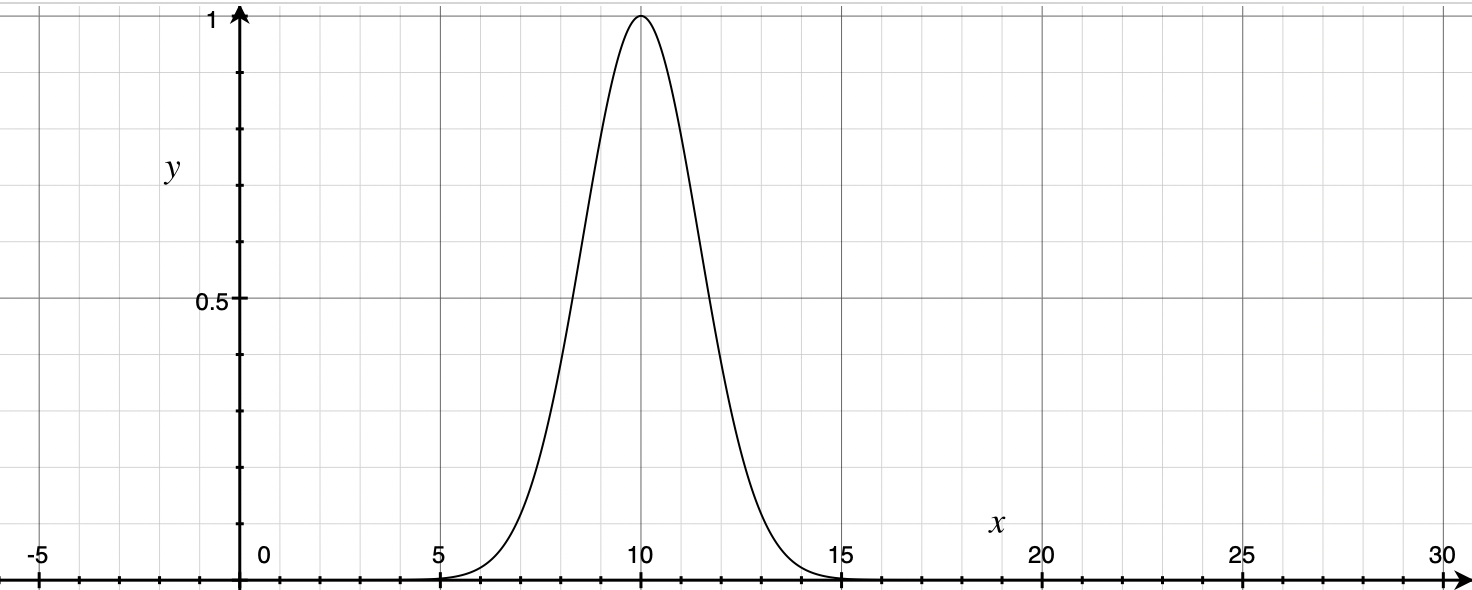
\includegraphics[width=0.8\textwidth]{graph1}
	\caption{Функция принадлежности нечеткого множества, соответствующего точечной оценке \textit{ПРИБЛИЗИТЕЛЬНО 10}}
	\label{fig:graph1}
  \end{figure}

\subsection{Построить функцию принадлежности нечеткого множества, соответствующего интервальной оценке \textit{ПРИБЛИЗИТЕЛЬНО В ИНТЕРВАЛЕ ОТ $K$ ДО $L$}}

Имеем оценку $X$ находится \textit{ПРИБЛИЗИТЕЛЬНО В ИНТЕРВАЛЕ ОТ $10$ ДО $15$}. 
На этом интервале функция принадлежности равна единице, а за его пределами будет повторять функции принадлежности, соответствующие точечным оценкам \textit{$X$ ПРИБЛИЗИТЕЛЬНО РАВЕН $10$} и \textit{$X$ ПРИБЛИЗИТЕЛЬНО РАВЕН $15$} слева и справа от интервала. Для построения функции принадлежности нечеткого множества, соответствующего интервальной оценке, необходимо дважды воспользоваться описанным выше методом.

Для \textit{$X$ ПРИБЛИЗИТЕЛЬНО РАВЕН $10$} формулу возьмем из предыдущих расчетов: 
\[
	y_1(x_1) = e^{-0.2388(10 - x_1)^2}.
\]

Для \textit{$X$ ПРИБЛИЗИТЕЛЬНО РАВЕН $15$} произведем расчет параметров $\alpha$ и $k$: 
\[
	y_2(x_2) = e^{-\alpha(k - x_2)^2}.
\]

Определяем значение переменных $q$, $r_q$, $r_{q+1}$ и $d$. Младшая значащая цифра числа $L$ стоит в разряде единиц, т.е. имеем $q=1$; $r_1$ = $5$ --- младшая значащая цифра числа $K$; $r_2 = 1$ --- цифра, имеющая порядок на единицу выше порядка младшей значащей цифры.

При делении числа $q$ на $3$ в остатке получаем $1$, т.е. число $К$ принадлежит к классу эквивалентности $M_1$ и переменная $d$ получает значение единицу. 

Тогда $z=r_2 \cdot 10 + r_1=15$, $\beta(L) = \beta(q)\cdot 10^{q-1} = 6.48$

Известно что функция принимает значение $y_2(15)=1$, $y_2(15-\beta(L)/2)=y_2(11.76)=y_2(a)=0.5$, a $k = 15$.

Найдем значение переменной $\alpha$:
\begin{align*}
	\ln y_(a) &= -\alpha(k - a)^2, \\
	\ln 0.5 &= -\alpha(15 - 11.76)^2, \\
	\ln 0.5 &= -\alpha \cdot 3.24^2, \\
	\alpha = - \frac{\ln 0.5}{3.24^2} &= - \frac{\ln 0.5}{10.4976} = 0.0660.
\end{align*}

Для \textit{$X$ ПРИБЛИЗИТЕЛЬНО РАВЕН $15$} формула будет иметь вид: 
\[
	y_2(x_2) = e^{-0.0660(15 - x_2)^2}.
\]

Окончательная формула имеет вид, график ее предствален на рисунке~\ref{fig:graph2}:
\[
	y(x) = 
	\begin{cases} 
		e^{-0.2388(10 - x)^2}, & \mbox{если } x \leq 10 \\ 
		e^{-0.0660(15 - x)^2}, & \mbox{если } x \geq 15 \\
		1.
	\end{cases}
\]

\begin{figure}[H]
	\centering
	  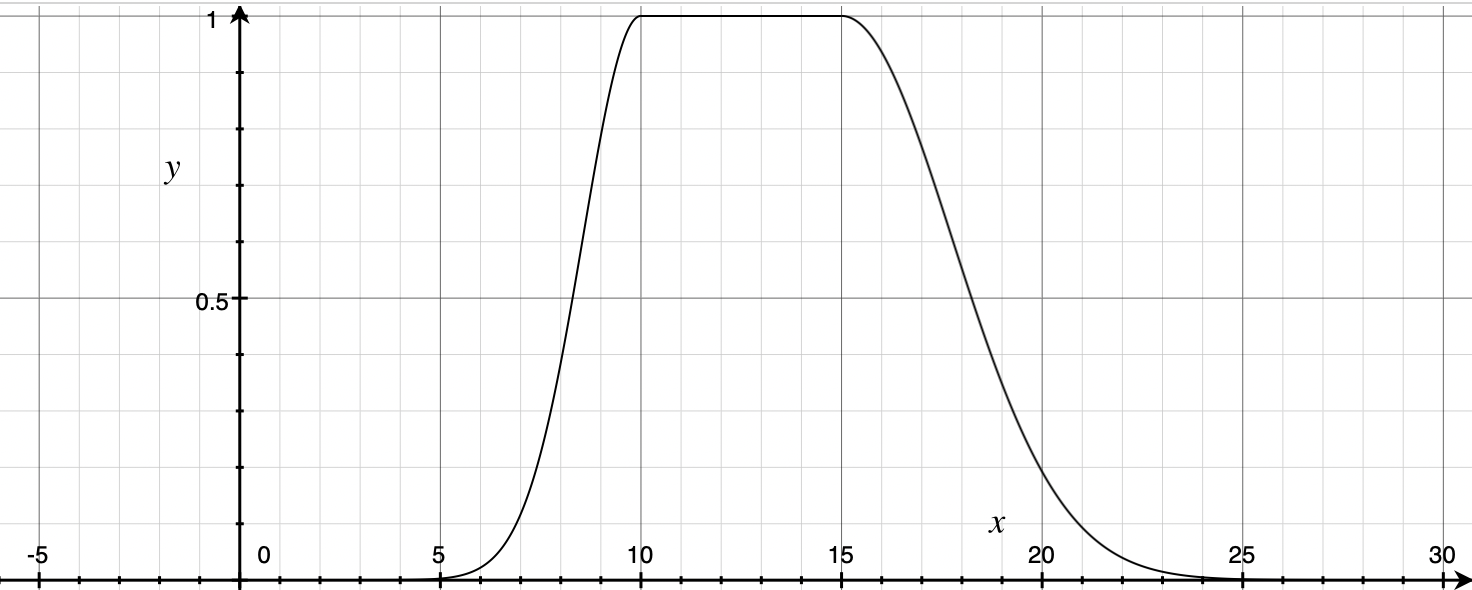
\includegraphics[width=0.8\textwidth]{graph2}
	\caption{Функция принадлежности нечеткого множества, соответствующего точечной оценке \textit{ПРИБЛИЗИТЕЛЬНО В ИНТЕРВАЛЕ ОТ $10$ ДО $15$}}
	\label{fig:graph2}
  \end{figure}

\subsection{Выводы}

В ходе лабораторной работы был изучен метод построения функций принадлежности на основе экспертных оценок, решена практическая задача в соответствии с методом построения функций принадлежности на основе экспертных оценок.

\end{document}
